\section{Limits and Continuity}

%% Flesh out continuity and add more expositon, provide an involved example of where one might to use a limit

In the previous example, we saw that zooming in and only looking at the average speed for small time intervals can help us figure out the speed at a particular moment in time, but we still don't know exactly how close we have to zoom to guarantee the right answer. This leads us to the concept of limits.\\

Conceptually a limit asks, \emph{what happens to our function when you get very close to a certain point?}. Looking at our previous example, we zoomed in on $t^*$ to find the limit of $\frac{\Delta x}{\Delta t}$ as $\Delta t$ got small or \emph{approaches 0}. This is idea behind a limit. Since the position of the runners changed in time, we were able to `zoom in' on a particular time to find how fast they were moving at that instant.

\subsection{Preliminaries \& Limit Definitions}

Before moving for let's look at this more abstractly and develop some notation for dealing with these questions. From the discussion above, we can see that we're interested in functions of some kind of \emph{variable} like time, position, height, energy, population, dollars or whatever quantity you might think of. That is, if we have a number $x$ representing a quantity like this, we want to assign it to another number $f(x)$.  We'll call the rule $f$ which takes $x\mapsto f(x)$ a \emph{function}. Usually, we'll just write $x\in\bbR$ to say that $x$ is a \emph{real number} like the ones we encounter in everyday life. 1,2,3, $\frac{2}{3}$, 1.21, and 3.14 for example. With this in mind, since the function $f$ takes real numbers to real numbers, we can write it as
\[
f\colon \bbR \to \bbR.
\] Alternatively, if $f$ isn't defined for all numbers $\bbR$, but only some subset of numbers $A$, we can write that $f\colon A\to\bbR$. This means that $f$ takes $x$ in $A$ to $f(x)\in\bbR$. These sets $A$ are usually `nice' sets like \emph{open interval} $(a,b)$ i.e. the set of real numbers that are between $a$ and $b$ or
\[
(a,b)=\{x\in\bbR \mid a<x<b \}
\]
or the closed interval which includes the endpoints
\[
[a,b]=\{x\in\bbR \mid a\leq x\leq b \}.
\]

\begin{rem}
  The brackets $\{\cdot \}$ used above are used to denote a \emph{set} and we often use set notion to denote a `container' of objects as a way of simplify our notion. For example, we'll write $\{y\mid C \}$ to denote the collection of objects $y$ that satisfy a condition $C$. We'll say that $x\in \{y\mid C \}$ to mean that $x$ is an element of our set i.e. that $x$ satisfies the condition $C$. %%Maybe turn into appendix of set notion.
\end{rem}
Let's we reframe this limit idea in this fancy new notation.
If we have a function $f\colon A\to \bbR$ and want to find the limit as $x$ approaches $a$ to exist, then we want $f(x)$ to approach a single number as we get close to our point $a$. In order to get at what this means mathematically, we need something called the \emph{absolute value} or \emph{norm}, which is what mathematicians use to measure magnitudes and distances. As you will see, the absolute value follows most of the same rules you would expect of distances in real life.

\begin{defn}[Absolute Value]
The absolute value of a number $a$ is defined by:
\begin{equation}
	\abs{a}=\begin{cases}
		a &\ \text{if}\ a\geq 0\\
		-a &\ \text{if}\ a<0.
\end{cases}
\end{equation}
\end{defn}

 We can think as the absolute value as function that takes in a number and returns the positive part. For example, $\abs{-3}=3$. In this way, it is similar to distance. In real life, if you move 5 feet to the left or to the right, you still moved 5 feet; the only difference is \emph{direction}. Therefore, the absolute value is only concerned with the \emph{magnitude} or \emph{total distance} traveled by saying that moving 5 feet in any direction is the same in terms of distance. Similarly, we say that the distance between two points $x$ and $a$ is given by $\abs{x-a}$. We can use inequalities to illustrate this. What if I ask you to solve the inequality
 \begin{equation*}
 	\abs{x-4}<7.
\end{equation*}
We can solve this by noticing that if $\abs{x-4}<7$, then both $x-4<7$ and $4-x<7$, so $x-4>-7$. Doing some work with inequalities, we see that
\begin{equation}
  -7<x-4<7
  \implies-3<x<11.
\end{equation}
We can visualize this on a number line.\\
\begin{figure}
  \centering
	\begin{tikzpicture}[scale=0.75]
		\draw[<->] (-6,0) -- (13,0);
	%	\draw[thick] (0,0.1)-- (0,-0.1);
		\draw[thick] (-3,0.1)-- (-3,-0.1);
		\draw[thick] (11,0.1)-- (11,-0.1);
		\draw[thick] (4,0.1)-- (4,-0.1);

		\node at (-3, -0.1) [below] {$-3$};
		\node at (4, 0) [below] {$4$};
		\node at (11, -0.1) [below] {$11$};

		\draw[thick, cyan, (-)] (-3,0) -- (11,0);
	\end{tikzpicture}\caption{$\abs{x-4}<7$ on the number line.}
\end{figure}

The absolute value has several interesting properties that are consistent with our interpretation of it as distance.

\begin{prop}[Properties of Absolute Value]\leavevmode
	For any numbers $x$ and $y$
\begin{enumerate}
	\item $\abs{x}=0$ if and only if $x=0$,
	\item $\abs{x}=\abs{-x}$,
	\item $\abs{xy}=\abs{x}\abs{xy}$,
	\item $\abs{x^2}=\abs{x}^2=x^2$,
	\item $\abs{x+y}\leq\abs{x}+\abs{y}$.
\end{enumerate}
\end{prop}

The last property is called the \emph{triangle inequality} and will prove to be very useful in establishing some of the properties of limits.\\

%% Add more about absolute value

%% Do one more example and add two exercises?


With an idea of distance and closeness at hand, we can revisit the question of \emph{what happens to our function when you get very close to a certain point?}. Let's say we have a function $f\colon A\to \bbR$ and a point $a$. If we want to find the \emph{limit of $f$ as $x$ approaches $a$}, we want to find a number $L\in\bbR$ such that \emph{$f(x)$ approaches $L$ when $x$ approaches $a$}. If we can find a number like this, we write
\begin{equation}
	\lim_{x\to a}f(x)=L.
\end{equation}
\begin{defn}\label{EpsDeltaDef}
	Formally, we define this by
	\begin{equation}
		\lim_{x\to a}f(x)=L
	\end{equation}
if for every $\epsilon>0$, there exists $\delta>0$ such that
\begin{equation*}
\abs{x-a}<\delta \implies \abs{f(x)-L}< \epsilon.
\end{equation*}
\end{defn}
\begin{rem}
  In words, we would say `the limit of $f$ as $x$ approaches $a$ is equal to $L$'.
\end{rem}

This is an example of a `$\epsilon$-$\delta$' statement which can be very difficult to unpack when you first see.To help give the notation above meaning, we attempt to visualize this $\epsilon$-$\delta$ definition of a limit in \cref{fig:EpDelta} below.

\begin{figure}\label{fig:EpDelta}
\centering
\hspace{-6mm}
\begin{subfigure}{0.35\textwidth}
  \centering
  \begin{tikzpicture}[scale=.5]
    \draw [<->] (0,10)--(0,0)-- (10,0);
    \draw[thick] (5, 0.1) -- (5, -0.1);
    \draw[thick] ( 0.1,5) -- (-0.1,5);
    \draw[thick, cyan, (-)] (0,4)--(0,6);

\node at (5,0) [below] {$a$};
\node at (0,5) [left] {$L$};
\node at (0,4) [left] {$L-\epsilon$};
\node at (0,6) [left] {$L+\epsilon$};

\draw[dashed] (0,4)-- (10,4);
\draw[dashed]	(0,6)-- (10,6);

\draw[thick, domain=0:7.5] plot (\x, {\x});
\draw[fill=white] (5, 5) circle [radius=0.2];
  \end{tikzpicture}
  \caption{For every $\epsilon>0$,}
\end{subfigure}\hfill%
\begin{subfigure}{0.35\textwidth}
  \centering
\begin{tikzpicture}[scale=.5]
	\draw [<->] (0,10)--(0,0)-- (10,0);
	\draw[thick] (5, 0.1) -- (5, -0.1);
	\draw[thick] ( 0.1,5) -- (-0.1,5);
	\draw[thick, cyan, (-)] (0,4)--(0,6);
  \draw[thick, cyan, (-)] (3,0)--(7,0);

\node at (5,0) [below] {$a$};
\node at (0,5) [left] {$L$};
\node at (3,0) [below] {$a-\delta$};
\node at (7,0) [below] {$a+\delta$};

\draw[dashed] (0,4)-- (10,4);
\draw[dashed]	(0,6)-- (10,6);

\draw[thick, domain=0:7.5] plot (\x, {\x});
\draw[fill=white] (5, 5) circle [radius=0.2];
\end{tikzpicture}
\caption{there exists $\delta>0$ such that}
\end{subfigure}
\vspace{5mm}
\begin{subfigure}{0.35\textwidth}
  \centering
\begin{tikzpicture}[scale=.5]
	\draw [<->] (0,10)--(0,0)-- (10,0);
	\draw[thick] (5, 0.1) -- (5, -0.1);
	\draw[thick] ( 0.1,5) -- (-0.1,5);
	\draw[thick, cyan, (-)] (0,4)--(0,6);
	\draw[thick, cyan, (-)] (3.5,0)--(6.5,0);

	\draw[thick] (4.3, 0.1) -- (4.3, -0.1);
	\node at (4.3, 0) [below] {$x$};
	\draw[dashed] (3.5,0)-- (3.5,10);
	\draw[dashed]	(6.5,0)-- (6.5,10);
	\draw[dotted] (4.3,0)-- (4.3, 10);

	\node at (5,0) [below] {$a$};
	\node at (0,5) [left] {$L$};

	\draw[dashed] (0,4)-- (10,4);
	\draw[dashed]	(0,6)-- (10,6);

	\draw[thick, domain=0:7.5] plot (\x, {\x});
	\draw[fill=white] (5, 5) circle [radius=0.2];
\end{tikzpicture}
\caption{if $\abs{x-a}<\delta$, }
\end{subfigure}\hfill%
\begin{subfigure}{0.35\textwidth}
  \centering
  \begin{tikzpicture}[scale=.5]
  		\draw [<->] (0,10)--(0,0)-- (10,0);
  		\draw[thick] (5, 0.1) -- (5, -0.1);
  		\draw[thick] ( 0.1,5) -- (-0.1,5);
  		\draw[thick, cyan, (-)] (0,4)--(0,6);
  		\draw[thick, cyan, (-)] (3.5,0)--(6.5,0);

  		\draw[thick] (4.3, 0.1) -- (4.3, -0.1);
  		\node at (4.3, 0) [below] {$x$};

  		\draw[dashed] (3.5,0)-- (3.5,10);
  		\draw[dashed]	(6.5,0)-- (6.5,10);
  		\draw[dotted] (4.3,0)-- (4.3, 10);

  		\node at (5,0) [below] {$a$};
  		\node at (0,5) [left] {$L$};

  		\draw[thick] ( 0.1,4.3) -- (-0.1,4.3);
  		\node at (0,4.3) [left] {$f(x)$};

  		\draw[dashed] (0,4)-- (10,4);
  		\draw[dashed]	(0,6)-- (10,6);
  		\draw[dotted] (0,4.3)-- (10, 4.3);

  		\draw[thick, domain=0:7.5] plot (\x, {\x});
  		\draw[fill=white] (5, 5) circle [radius=0.2];
  \end{tikzpicture}
  \caption{then $\abs{f(x)-L}<\epsilon$.}
\end{subfigure}

\caption{Visualizing the $\epsilon$-$\delta$ definition.}
\end{figure}

Intuitively, this is saying that if $\lim\limits_{x\to a}f(x)=L$, then our function $f$ can get close as we want to some value $L$ if we zoom in close enough to $a$ i.e. if $f(x)\approx L$ whenever $x\in(a-\delta,a+\delta)$ for some small number $\delta$.\\

Be fair warned, not all functions have proper limits everywhere! Take
\[
g(x)=\begin{cases}
  1 & \text{if } x\geq 0\\
  0 & \text{if }  x<0,
\end{cases} %% Graph this function below.
\]for example! If we graph this function, we'll see that it clearly has no limit at 0. Before moving on to some of the interesting properties of limit, let's show an example of how to use the $\epsilon-\delta$ definition to prove a limit exists.
\begin{exmp}
  Calculate $\lim\limits_{x\to 2} (3x-1)$ and prove your result. \\

Looking at the graph of $f(x)=3x-1$, you can see that $\lim\limits_{x\to 2} 3x-1=5$, but in order to \emph{prove} this, we must use the $\epsilon$-$\delta$ definition.\\

Suppose we have some small number $\epsilon>0$. If the limit exists, then we know that if we zoom in close enough to $a=2$ on the $x$-axis that our function $f(x)=3x-1$ will be $\epsilon$ close to the limit $L=5$. The point of $\delta$ is to tell us how close we need to be to $a=2$ so that $f(x)=3x-1$ is $\epsilon$-close to $5$. Let's show this mathematically in terms of \cref{EpsDeltaDef}.\\

\begin{figure}
  \centering
\begin{tikzpicture}[scale=.7]
		\draw [<->] (0,10)--(0,0)-- (10,0);
		\draw[thick] (5, 0.1) -- (5, -0.1);
		\draw[thick] ( 0.1,5) -- (-0.1,5);
		\draw[thick, cyan, (-)] (0,4)--(0,6);
		\draw[thick, cyan, (-)] (3.5,0)--(6.5,0);

		\draw[thick] (4.3, 0.1) -- (4.3, -0.1);
		\node at (3.5, 0) [below] {$2-\delta$};
    \node at (6.5, 0) [below] {$2+\delta$};


		\draw[dashed] (3.5,0)-- (3.5,10);
		\draw[dashed]	(6.5,0)-- (6.5,10);
		\draw[dotted] (4.3,0)-- (4.3, 10);

		\node at (5,0) [below] {$2$};
		\node at (0,5) [left] {$5$};

		\node at (0,4) [left] {$f(x)-\epsilon$};

    \node at (0,6) [left] {$f(x)+\epsilon$};

		\draw[dashed] (0,4)-- (10,4);
		\draw[dashed]	(0,6)-- (10,6);
		\draw[dotted] (0,4.3)-- (10, 4.3);

		\draw[thick, domain=0:7.5] plot (\x, {\x});
		\draw[fill=white] (5, 5) circle [radius=0.2];
\end{tikzpicture}
\caption{Visualizing the argument above.}
\end{figure}

We see that if $f(x)$ is $\epsilon$-close to $5$, we can write this mathematically as
\[
\abs{f(x)-5}<\epsilon.
\]
If we substitute in the definition of $f(x)$, we see
\[
\abs{(3x-1)-5}=\abs{3x-6}<\epsilon,
\]
but what we want to find is a number $\delta$, so that if $x$ is $\delta$-close then $f(x)$ is $\epsilon$-close to 5! We can write $x$ is $\delta$-close to $2$ as
\[
\abs{x-2}<\delta.
\]
If you compare the two inequalities above, you see that you can make the lefthand sides equal by multiplying by $3$ which shows
\[
3\abs{x-2}= \abs{3x-6}=\abs{3x-1)-5} <3\cdot\delta.
\]
From this, we see that if $\delta=\frac{\epsilon}{3}$, then
\[
\abs{3x-6}<3\cdot\delta=3\cdot\frac{\epsilon}{3}=\epsilon,
\]
which gives us the inequality we want to see! With this information, we can write the proof as follows.
\begin{proof}
  Let $\epsilon>0$ and $\delta=\frac{\epsilon}{3}$. If
  \[
\abs{x-2} < \delta,
  \]
  then after multiplying by 3, we see
  \[
\abs{3x-6} < \epsilon.
  \]
  Therefore,
  \[
    \abs{3x-6}=\abs{(3x-1)-5} =\abs{f(x)-5 }<\epsilon,
    \]
which proves that the limit is equal to 5.
\end{proof}
\end{exmp}


%% Add left hand and right hand limits


%% A limit exists if and only if the left and righthand limits exist and are equal

%% \begin{thm}
%%  If $\lim\limits_{x\to a^{-}}f(x)=L$ and $\lim\limits_{x\to a^{+}}f(x)=L$, then $\lim\limits_{x\to a}f(x)=L$
%% \end{thm}

%% Piecewise example

%% Difference between limit DNE and function undefined

The idea of limits is conceptually robust and natural, but when it comes to most of applications we're interested in, we'll encounter more complicated functions which make this approach either extremely difficult or just tedious. Because of this,  we'll develop some methods of computing complicated limits using simpler functions which we already know the limit of. For example, if we have two functions $f$ and $g$ which have limits $L$ and $M$, it's reasonable to assume that $f+g$ converges to $L+M$ (why?). Is this also true for $f\cdot g$ or $10\cdot f$? We'll provide an answer to these questions with the following with the following theorems.

\subsection{Limit Theorems}

\begin{thm}[Properties of Limits]\label{LimRules}
If the limits of two functions $f(x)$ and $g(x)$ exist at $a$. That is, if $\lim\limits_{x\to a}f(x)=L$ and $\lim\limits_{x\to a}g(x)=M$ for some numbers $L$ and $M$, then
	\begin{enumerate}
		\item $\lim\limits_{x\to a}\left[f(x)+g(x)\right]=L+M$,
		\item $\lim\limits_{x\to a}\left[cf(x)\right]=cL$ if $c$ is any number,
		\item  $\lim\limits_{x\to a}\left[f(x)\cdot g(x)\right]=L\cdot M$,
		\item if $M\neq 0$, $\lim\limits_{x\to a}\frac{f(x)}{g(x)}=\frac{L}{M}$.
		\end{enumerate}
\end{thm}

As you can see, these rules make calculating limits like
\begin{equation}
\lim\limits_{x\to 3}\frac{x^2-1}{x^8-3x}
\end{equation}
much easier. In this case, it's as simple as plugging in 3 into our equation, but it won't always be this easy. We'll formalize this idea of functions are `nice' and  `not-so-nice' to evaluate with limits in the next sections as we develop the ideas of \textit{continuity} and \textit{differentiblity}.\\

%% Move onto the left and right hand derivatives?

Conceptually, we say that a function is continuous if we `can draw its graph without lifting our pencil`, but mathematically this means that if we move a tiny little on the $x$-axis then we also move a tiny bit up or down on the graph of our function. Let's try and write this idea in terms of limits.

\begin{defn}
We say that a function $f(x)$ is \emph{continuous at $a$} if \begin{equation}
	\lim\limits_{x\to a}f(x)=f(a).
\end{equation}
If $f(x)$ is continuous at every point it is defined, then we just say that $f(x)$ is continuous.
\end{defn}

As you might expect, not all functions are continuous, take $\frac{1}{x}$ for example. This fails to be continuous at $0$.

The limit properties described earlier are useful for determining continuity.
\begin{thm}
	If $f$ and $g$ are continuous at $a$, then
	\begin{enumerate}
		\item $f+g$, $f\cdot g$ are continuous at $a$,
		\item $cf$ is continuous at $a$ for any real number $c$,
		\item $\frac{f}{g}$ is continuous at $a$ whenever $g(a)\neq 0$.
	\end{enumerate}
\end{thm}

We also have another property for the composition of continuous functions.

\begin{thm}
	If $f$ is continuous at $a$ and $g$ is continuous at $f(a)$, then $g\circ f$ is continuous at $a$.
\end{thm}


There are other properties of limits and continuity such as the squeeze and intermediate value theorems! We'll begin with the squeeze theorem.

\begin{thm}[Squeeze Theorem]
  Suppose $f(x)$ is defined near $c$, and there are functions $U(x)$ and $L(x)$ which bound $f(x)$ near $c$ i.e.
  \[
L(x)\leq f(x)\leq U(x)\text{ for every }x\text{ near }c.
  \]
  If $\lim\limits_{x\to c} U(x)= \lim\limits_{x\to c} L(x)$, then
  \[
  \lim\limits_{x\to c} L(x)=\lim\limits_{x\to c} f(x) =\lim\limits_{x\to c} U(x).
  \]
\end{thm}

  This is the statement that if $f(x)$ is sandwiched between two functions $L(x)$ and $U(x)$ that approach each other, then $f(x)$ must approach their common value. We can see an application of this theorem in the following example.

  \begin{figure}[h]
    \centering
    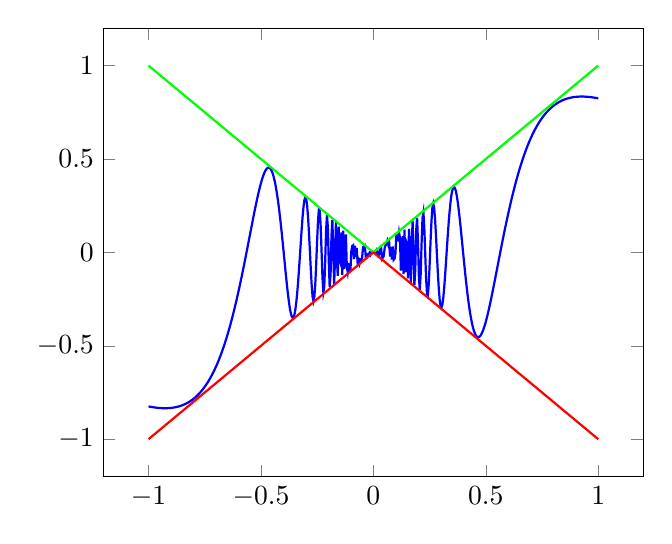
\begin{tikzpicture}
    \begin{axis}[samples=500,domain=-1:1,restrict y to domain =-1:1]
    \addplot[thick,blue ]plot (\x, {0.98*\x*sin(pow(\x,-2) r)});
    \addplot[thick,green]plot (\x, {abs(\x)});
    \addplot[thick,red]plot (\x, {-abs(\x)});
    \end{axis}
    \end{tikzpicture}
    \label{fig:Squeeze}
    \caption{Graphs of $f(x)=x\sin\left(\frac{1}{x^2}\right), L(x)=-\abs{x}|, U(x)=\abs{x}$.}
  \end{figure}


\begin{exmp}
  What is the limit of $f(x)=x\sin\left(\frac{1}{x^2}\right)$ as $x$ approaches 0?\\

  Graphing the function ( \cref{fig:Squeeze}), we see that as we zoom into the origin, $f(x)$ appears to approach zero. We can see this analytically by considering the absolute value of $f(x)$ as follows

  \begin{align}
    \abs{f(x)}&=\abs{x\sin\left(\frac{1}{x^2}\right) }\\
    &= \abs{x}\cdot\abs{\sin\left(\frac{1}{x^2}\right) }.
  \end{align}

The part of interest here is the $\sin\left(\frac{1}{x^2}\right)$. One might remember from pre-calculus that $\sin(\theta)$ is bounded between $1$ and $-1$ for every number $\theta$. Therefore, we see that
\[
\abs{f(x)}\leq \abs{x}\text{ for any }x \text{ near }0.
\]
Breaking down the absolute value around $f(x)$, then gives us

\[
-\abs{x}\leq f(x)\leq \abs{x}\text{ for any }x \text{ near }0.
\]
Therefore, we have functions $U(x)=\abs{x}$ and $:(x)=-\abs{x}$ such that
\[
\lim\limits_{x\to 0} U(x)=\lim\limits_{x\to 0} L(x)= 0
\]
which bound $f(x)$ near 0. Therefore, by Squeeze Theorem, we now know that
\[
\lim\limits_{x\to 0}x\sin\left(\frac{1}{x^2}\right)=0.
\]
\end{exmp}

Another useful theorem involving limits and continuity is the Intermediate Value Theorem!

\begin{thm}[Intermediate Value Theorem]
  Suppose $f$ is continuous on an interval $[a,b]$ and $M$ is a number between $f(a)$ and $f(b)$, then there is some point $c$ between $a$ and $b$ such that $f(c)=M$.
\end{thm}
The intuition behind this relies on the fact that if a function is continuous, then it has no `hops,skips, breaks, or jumps'. Therefore, for a continuous function to go from greater than $M$ to less than $M$, the function must pass through $M$ at some point!\\

We can use the Intermediate Value Theorem to show the existence of roots for a given function.

\begin{exmp}
Show that $f(x)=3x^3+x^2-x-\frac{1}{8}$ has a root.\\

\begin{figure}
  \centering
  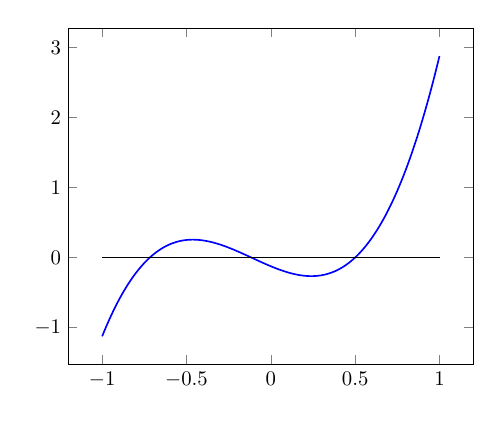
\begin{tikzpicture}[scale=0.75]
  \begin{axis}[samples=500,domain=-1:1,restrict y to domain =-1.25:3]
  \addplot[thick,blue ]plot (\x, {3*\x*\x*\x+\x*\x-\x-1/8});
  \addplot[thin,black ] plot (\x, {0});
  \end{axis}
  \end{tikzpicture}
  \caption{Graph of $f(x)=3x^3+x^2-x-\frac{1}{8}$ on $[0,1]$}
\end{figure}

Let's consider $f$ on the interval $[-1,1]$. We can compute that $f(-1)=-1-\frac{1}{8}$ and $f(1)=3-\frac{1}{8}$. We notice that
\[
f(-1)<0<f(1).
\] Since $f(x)$ is continuous, we can apply the Intermediate Value Theorem which tells us that there is some point $c$ between $0$ and $1$ such that $f(c)=0$. This, however, doesn't answer the question of how many roots $f(x)$ has in $[0,1]$. The Intermediate Value Theorem guarantees that there is at least one root of $f$. If we graph $f(x)$, we see that it actually has 3 roots in $[0,1]$.
\end{exmp}

%% Talk about intermediate value theorem use some polynomial as example of having multiple roots but only showing existence of a root!

%% Let's see another way this can be apply
%% Bower's fixed point theorem if f takes interval to itself it has a fixed points

%% A population grows by ,,,, we want to know if there's a stable population

%% Discrete logistic map, rx(1-x)m we can see that the max of this is r/4

%% Later, we'll be able to show that the maximum is

%% Later, we can see whether or not the population will actually approach the fixed point

%% How does the equilibrium change with the fertility r.


We now move onto the actual definition of differentiability, so that we can answer our question about how to find the rate of change of a function at a given point.
